\documentclass{article}

%%%%%%%%%%%%%%%%%%%%%%%%%%%%%%%%%%%%%%%%%%%%%%%%%%%%%%%%%%%%%%%%%%%%%%%%%%%%%%%%%%
\usepackage{url}
\usepackage[breaklinks]{hyperref}
\usepackage{breakurl}

\usepackage{graphicx}

\usepackage[svgnames]{xcolor} 

\usepackage{amsmath}
\usepackage{amsfonts}
\usepackage{amssymb}

\usepackage[top=2.5cm, bottom=2.5cm, left=2.5cm, right=2.5cm]{geometry}

\usepackage{comment}
%%%%%%%%%%%%%%%%%%%%%%%%%%%%%%%%%%%%%%%%%%%%%%%%%%%%%%%%%%%%%%%%%%%%%%%%%%%%%%%%%%
\usepackage[
backend=biber,
style=alphabetic,
sorting=ynt
]{biblatex}
\addbibresource{bibliografia.bib}


%%%%%%%%%%%%%%%%%%%%%%%%%%%%%%%%%%%%%%%%%%%%%%%%%%%%%%%%%%%%%%%%%%%%%%%%%%%%%%%%%%
\newtheorem{theorem}{Theorem}%[section]
\newtheorem{mydef}{Definition}[section]
\newtheorem{corollary}{Corollary}[section]

% correct bad hyphenation here
\hyphenation{op-tical net-works semi-conduc-tor}

%%%%%%%%%%%%%%%%%%%%%%%%%%%%%%%%%%%%%%%%%%%%%%%%%%%%%%%%%%%%%%%%%%%%%%%%%%%%%%%%%%
% paper title
\title{ Error Reduction in the Tuning of Six Hole's Ocarina }

\author{Fernando Pujaico Rivera}

\date{ }

\begin{document}



% keywords: Resonator, Whistles, Helmholtz, ocarina
% make the title area
\maketitle


\begin{abstract}
In this paper we propose an optimal method for tuning a six hole's ocarina,
this optimization will be subordinated by the minimization of $|| \mathbf{\hat{f}}^2-\mathbf{f}^2||^2$, 
the square norm of square difference between the desired and obtained frequency.
The results show that it is not possible tuning a John Taylor style six hole's ocarina with an equal temperament scale,
but the method proposed here obtain an optimal approximation with heterogeneous errors less than $43.697\%$ of a semitone.
\end{abstract}



%%%%%%%%%%%%%%%%%%%%%%%%%%%%%%%%%%%%%%%%%%%%%%%%%%%%%%%%%%%%%%%%%%%%%%%%%%%%%%%%
%%%%%%%%%%%%%%%%%%%%%%%%%%%%%%%%%%%%%%%%%%%%%%%%%%%%%%%%%%%%%%%%%%%%%%%%%%%%%%%%
\section{Introduction}

The fingering style of the pendant-type ocarina was developed around 1964 
by the Engish mathematician John Taylor \cite[pp. 79]{metropolitan1985american} \cite[pp. 10]{galpin2001newsletter}.

%%%%%%%%%%%%%%%%%%%%%%%%%%%%%%%%%%%%%%%%%%%%%%%%%%%%%%%%%%%%%%%%%%%%%%%%%%%%%%%%
%%%%%%%%%%%%%%%%%%%%%%%%%%%%%%%%%%%%%%%%%%%%%%%%%%%%%%%%%%%%%%%%%%%%%%%%%%%%%%%%
\section{Fingering chart in  6 hole's ocarina}
The Fig. \ref{fig:ocarinaview} represents the hole distribution of the ocarina
used in this work, where $S_0$ represent the sound hole (voicing)
and the holes $S_1$, $S_2$, $S_3$, ... and $S_6$ represent the tone-holes.
\begin{figure}[ht!]
\centering
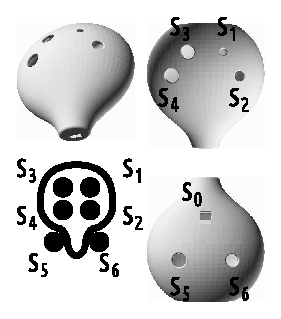
\includegraphics[width=0.50\columnwidth]{ocarina-view.eps}
\caption{View of 6 hole ocarina. }
\label{fig:ocarinaview}
\end{figure}
The fingering chart used in this ocarina model is based in the 
4 holes fingering style proposed by John Taylor \cite[pp. 79, 146]{metropolitan1985american}. In the
Table \ref{table:chart} we can see the fingering chart that indicates the configuration of open or close holes
to produce the tones from $C$ until $D$ (a higher octave ), where a value $S_i=1$ represents an
open hole and the value $S_i=0$ a closed hole.
\begin{table}[h!]
\center
\begin{tabular}{l|c|c|c|c|c|c}
Note & $S_1$ & $S_2$ & $S_3$ & $S_4$ & $S_5$ & $S_6$ \\ \hline
\hline 
$C$  & 0 & 0 & 0 & 0 & 0 & 0 \\
$C\#$& 0 & 0 & 0 & 0 & 0 & 1 \\
$D$  & 1 & 0 & 0 & 0 & 0 & 0 \\
$D\#$& 1 & 0 & 0 & 0 & 0 & 1 \\
$E$  & 0 & 1 & 0 & 0 & 0 & 0 \\
$F$  & 1 & 1 & 0 & 0 & 0 & 0 \\
$F\#$& 0 & 0 & 1 & 0 & 0 & 0 \\
$G$  & 1 & 0 & 1 & 0 & 0 & 0 \\
$G\#$& 0 & 1 & 1 & 0 & 0 & 0 \\
$A$  & 1 & 1 & 1 & 0 & 0 & 0 \\
$A\#$& 1 & 0 & 1 & 1 & 0 & 0 \\
$B$  & 0 & 1 & 1 & 1 & 0 & 0 \\
$C$& 1 & 1 & 1 & 1 & 0 & 0 \\
$C\#$& 0 & 1 & 1 & 1 & 1 & 0 \\
$D$& 1 & 1 & 1 & 1 & 1 & 0 \\ 
\hline 
\end{tabular}
\vspace{5pt}
\caption{Fingering chart}
\label{table:chart}
\end{table}

%%%%%%%%%%%%%%%%%%%%%%%%%%%%%%%%%%%%%%%%%%%%%%%%%%%%%%%%%%%%%%%%%%%%%%%%%%%%%%%%
%%%%%%%%%%%%%%%%%%%%%%%%%%%%%%%%%%%%%%%%%%%%%%%%%%%%%%%%%%%%%%%%%%%%%%%%%%%%%%%%
\section{Math and music}
In this paper we analyze a tuning method with 12 tone equal temperament; so that, the frequency interval
between any pair of adjacent notes has the same ratio $\rho = {\sqrt[12]{2}}$.
The Table \ref{tab:notes} shows how are distributed the musical notes from tone $C$ until $D$ (a higher octave ),
where $f_0$ represent the frequency of $C$ note and the next notes
follow the progression $\hat{f}_{i}={\rho}^i f_{0}$ with $i$ representing the separation degree with $C$. 

\begin{table}[h]
\center
{\renewcommand{\arraystretch}{1.5}
\begin{tabular}{|c|c|c|c|c|c|c|c|}
\hline
$\hat{f}_{0}$ & $\hat{f}_{1}$ & $\hat{f}_{2}$ & $\hat{f}_{3}$ & $\hat{f}_{4}$ & $\hat{f}_{5}$ & $\hat{f}_{6}$ & $\hat{f}_{7}$ \\ \hline
$C$ & $C\#$ & $D$ & $D\#$ & $E$ & $F$ & $F\#$ & $G$ \\ \hline
$f_{0}$ & ${\rho}^1 f_{0}$ & ${\rho}^2 f_{0}$ & ${\rho}^3 f_{0}$ & ${\rho}^4 f_{0}$ & ${\rho}^5 f_{0}$ & ${\rho}^6 f_{0}$ & ${\rho}^7 f_{0}$  \\ \hline
\hline 
$\hat{f}_{8}$ & $\hat{f}_{9}$ & $\hat{f}_{10}$ & $\hat{f}_{11}$ & $\hat{f}_{12}$ & $\hat{f}_{13}$ & $\hat{f}_{14}$ & ~ \\ \hline
$G\#$ & $A$ & $A\#$ & $B$ & $C$ & $C\#$ & $D$  & ~\\ \hline
${\rho}^8 f_{0}$ & ${\rho}^9 f_{0}$ & ${\rho}^{10} f_{0}$ & ${\rho}^{11} f_{0}$ & ${\rho}^{12} f_{0}$ & ${\rho}^{13} f_{0}$ & ${\rho}^{14} f_{0}$ & ~ \\ 
\hline
\end{tabular}
}
\vspace{5pt}
\caption{Musical notes}
\label{tab:notes}
\end{table}


\section{Math and ocarina}

\subsection{Analyzing a whistle}
We can think of an ocarina as a whistle with tone-holes in its resonant cavity,
so that when we open and close some of these holes we can modify the tone of generated sound.
Thus to understand the math of an ocarina first we should to know the science behind the whistles  
or more formally a Helmholtz resonant cavity \cite{corning2011resonance} (see Fig. \ref{fig:resonador}) excited by a jet-edge-resonator system (see Fig. \ref{football-referee-whistle}) \cite[pp. 3]{gibiat2013acoustic} \cite[pp. 138]{nyborg1953characteristics}. 
In this sense the Eq. \ref{eq:Apito} 
\begin{equation} 
\label{eq:Apito}
 f_0 = \frac{c}{2 \pi} \sqrt{\frac{A_{0}}{l_{0}V} }  
\end{equation}
shows the way of to calculate the frequency $f_0$ of a theoretic\footnote{A sphere-like resonant cavity and the open area of the neck is much less than the total surface area of the resonant cavity. .} whistle \cite[pp. 3]{gibiat2013acoustic} \cite[pp. 5]{kobayashi20093d} \cite[pp. 265]{okadanumerical}
in relation with the constants $\pi$  and $c$ (the velocity of sound),  and 
the variables: $V$ the volume of its resonant cavity,
$A_0$ is its cross-section area and $l_0$ the effective length of the neck in the resonator.


\begin{figure}[ht!]
\centering
\includegraphics[width=0.250\columnwidth]{resonador.eps}
\caption{whistle. }
\label{fig:resonador}
\end{figure}

\begin{figure}[ht!]
\centering
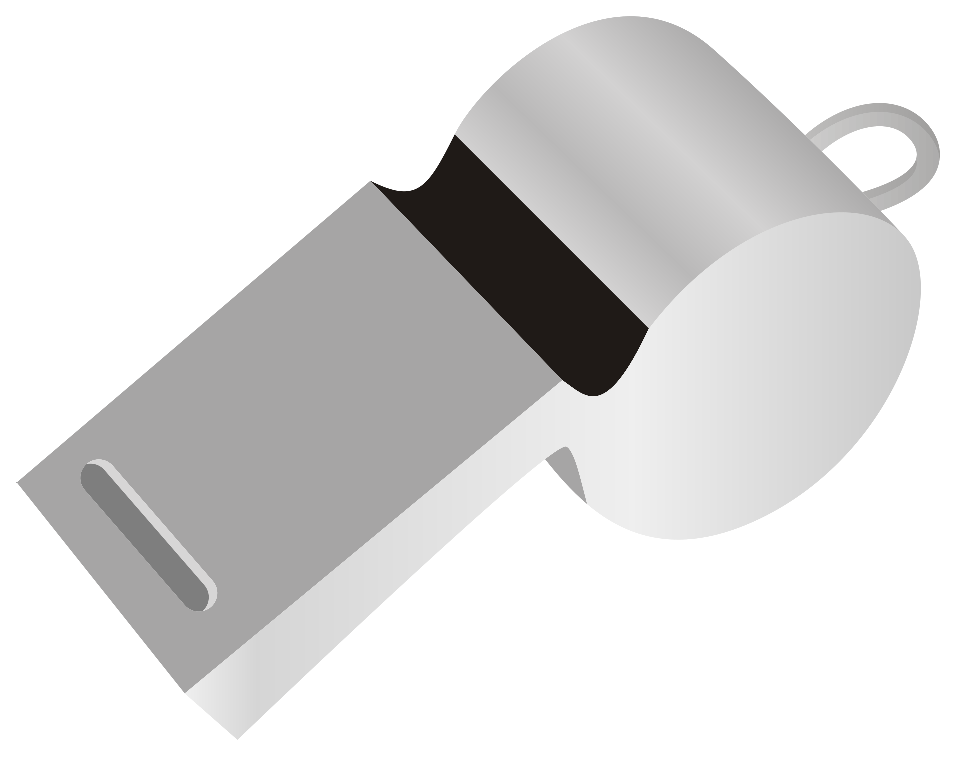
\includegraphics[width=0.250\columnwidth]{football-referee-whistle.eps}
\caption{whistle. }
\label{football-referee-whistle}
\end{figure}

\subsection{Analyzing an ocarina}

The fundamental resonant frequency $f$ of an ocarina, 
that have at least one circular tone-hole %pitch hole 
in addition to the sound hole (see Fig. \ref{fig:ocarina-teorica}),
can be represented like a function of the total tone-holes area $A$.


\begin{figure}[ht!]
\centering
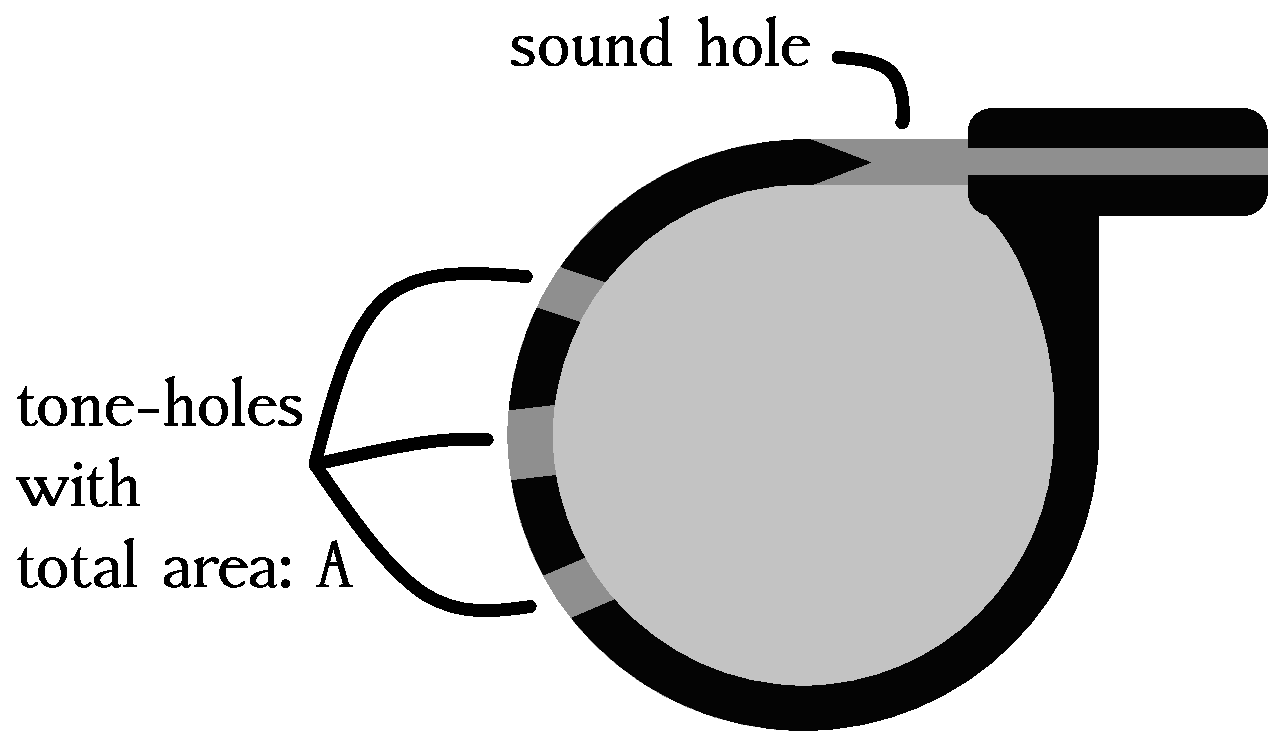
\includegraphics[width=0.350\columnwidth]{ocarina-teorica.eps}
\caption{Theoretic ocarina}
\label{fig:ocarina-teorica}
\end{figure}

In the article ``La Ocarina de Zanahoria a Carrot Ocarina'' \cite{mp2010ocarina}
were analyzed data about of the increment of resonant frequency $f$ in relation to the augment of area $A$,
showing that in that study case the relationships between the variables can be approximated with a line 
\begin{equation}
f=c_1+ c_2~A.
\end{equation}
where $c_1=595.859069$, $c_2=4.324273$ and a mean square error $MSE=8051.1$.
The Fig. \ref{fig:models} show the linear curve in relation to the collected data.


\begin{figure}[ht!]
\centering
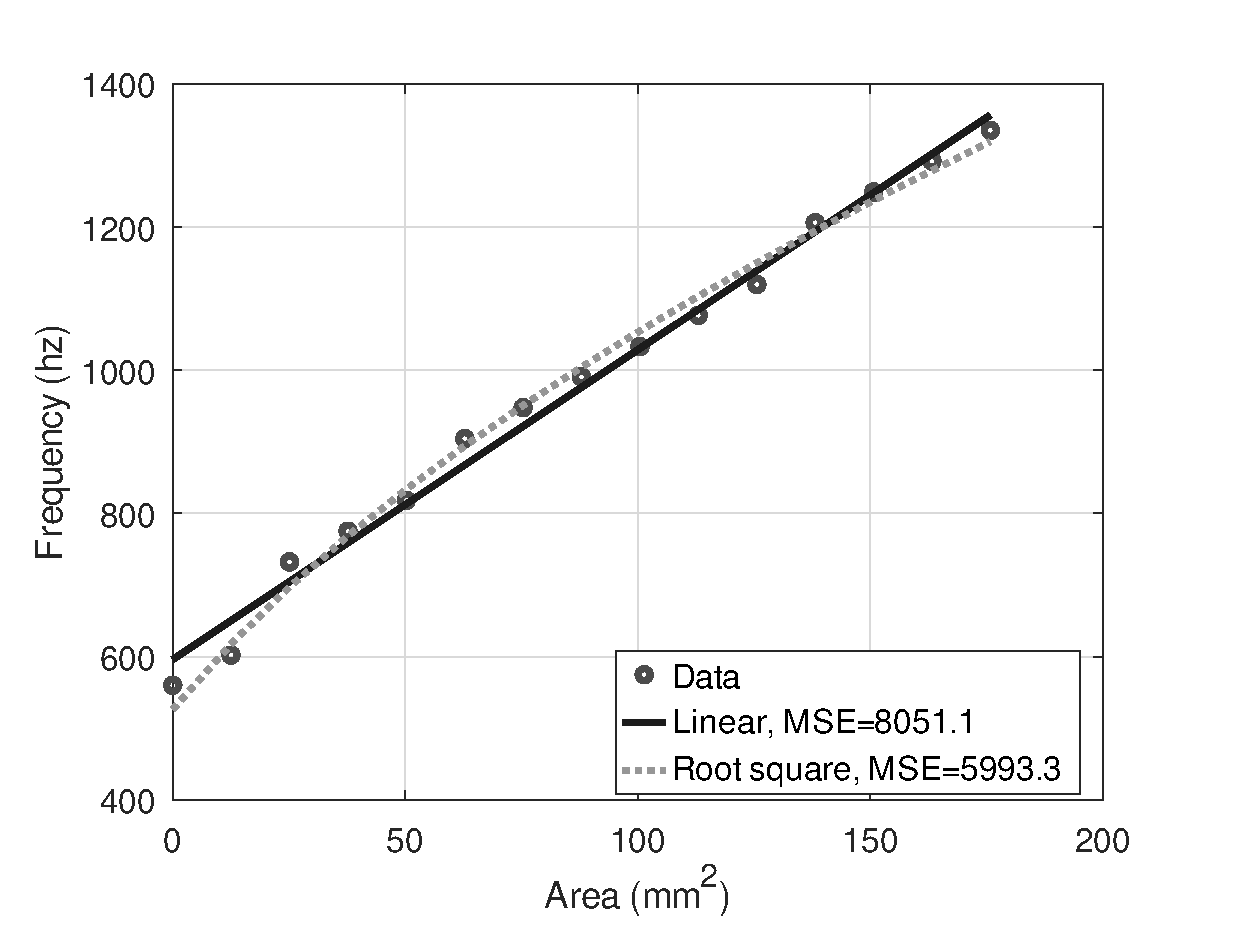
\includegraphics[width=0.50\columnwidth]{compara.eps}
\caption{Comparing models. }
\label{fig:models}
\end{figure}

By other side, 
if we follow the equation proposed by Bart Hopkin in its book ``Air Columns and Toneholes'' 
\cite[pp. 44]{cabreraestudio} \cite{1999air},
we can fit the data of Fig. \ref{fig:models} with a root square function
\begin{equation}
f=d_1\sqrt{d_2+A},
\end{equation}
where $d_1=91.215856$, $d_2=33.262474$ and a mean square error $MSE=5993.3$.
We must highlight that $d_2$ represents the area of sound hole. 

This last model fit better the data, 
also the equation proposed by Hopkin keep coherence with the Helmholtz resonator equation (see Eq. \ref{eq:Apito}).
In the next section we use the model proposed by Hopkin to obtain a optimal tuning in 
John Taylor style six hole's ocarina.


%%%%%%%%%%%%%%%%%%%%%%%%%%%%%%%%%%%%%%%%%%%%%%%%%%%%%%%%%%%%%%%%%%%%%%%%%%%%%%%%
%%%%%%%%%%%%%%%%%%%%%%%%%%%%%%%%%%%%%%%%%%%%%%%%%%%%%%%%%%%%%%%%%%%%%%%%%%%%%%%%
\subsection{Resonance frequency in ocarinas}


If we assume the equation \ref{EcA} proposed by Bart Hopkin \cite[pp. 44]{cabreraestudio} \cite{1999air},
\begin{equation} \label{EcA}
 f = \frac{c}{2 \pi} \sqrt{\frac{\frac{A_{0}S_{0}}{l_{0}}+\frac{A_{1}S_{1}}{l_{1}}+\frac{A_{2}S_{2}}{l_{2}}+ . . .}{V} }   
\end{equation}
as a good approximation to estimate the fundamental frequency $f$ 
of globular resonators that have at least one circular pitch hole in addition to the sound hole (a.k.a. an ocarina). 
in which $A_i$ and $l_i$ are the area an the effective length of the $S_i$ tone-hole,
so that the variable $S_i$ has only have two values $\{0,1\}$ according the Table \ref{table:chart},
additionally $S_0=1$ and represent the sound hole, being $A_0$ and $l_0$ their corresponding variables. 



\subsubsection{Reordering the resonance equation}

so that $h_{i}\propto \frac{A_{i}}{l_{i}}$
\begin{equation} \label{EcC}
 h_{i} =  \left( \frac{c^2}{4 {\pi}^2 V}\right) \left( \frac{A_{i}}{l_{i}}    \right) 
\end{equation}

\begin{equation} \label{EcD}
 f^{2} = \sum_{i=0}^{6}{S_i h_i}
\end{equation}

\begin{corollary}

\begin{equation} 
 f_0^{2} = h_0
\end{equation}
 
\end{corollary}



\section{Problem Statement}


\begin{mydef}[Square value of the desired frequencies]
Known the frequency relation between the notes showed in the Table \ref{tab:notes}, 
we define the variable $\hat{z}_i\equiv \hat{f}_i^2 \equiv \left( {\rho}^{i} f_0 \right)^{2} $,
so that the  column vector $\mathbf{\hat{z}}= \left[ \hat{z}_1, \hat{z}_2, \hdots, \hat{z}_{14}\right]^{T} $ 
that contain the square value of the desired frequencies
is represented as in the Eq. \ref{eq:vecz}.
\begin{equation} \label{eq:vecz}
\mathbf{\hat{z}}
\equiv \mathbf{P} f_{0}^2
\end{equation}

where $\mathbf{P}=[\rho^2,~\rho^4,~\rho^6,~\rho^8,~...,~\rho^{28}]^T$.

\end{mydef}

\begin{mydef}[Square value of the generated frequencies]
\begin{equation}
\mathbf{z}(\mathbf{h})
=  
\begin{bmatrix}
1 \\ 
1 \\ 
1 \\ 
1 \\ 
1 \\ 
1 \\ 
1 \\
1 \\ 
1 \\ 
1 \\ 
1 \\ 
1 \\ 
1 \\ 
1
\end{bmatrix}
h_{0} + 
\begin{bmatrix}
0 & 0 & 0 & 0 & 0 & 1 \\
1 & 0 & 0 & 0 & 0 & 0 \\
1 & 0 & 0 & 0 & 0 & 1 \\
0 & 1 & 0 & 0 & 0 & 0 \\ 
1 & 1 & 0 & 0 & 0 & 0 \\ 
0 & 0 & 1 & 0 & 0 & 0 \\
1 & 0 & 1 & 0 & 0 & 0 \\ 
0 & 1 & 1 & 0 & 0 & 0 \\ 
1 & 1 & 1 & 0 & 0 & 0 \\ 
1 & 0 & 1 & 1 & 0 & 0 \\ 
0 & 1 & 1 & 1 & 0 & 0 \\ 
1 & 1 & 1 & 1 & 0 & 0 \\
0 & 1 & 1 & 1 & 1 & 0 \\
1 & 1 & 1 & 1 & 1 & 0 
\end{bmatrix} 
\begin{bmatrix}
h_{1} \\
h_{2} \\
h_{3} \\
h_{4} \\
h_{5} \\
h_{6}
\end{bmatrix} 
\end{equation}


\begin{equation}
\mathbf{z}(\mathbf{h}) =  \mathbf{L}h_0 +  \mathbf{A} \mathbf{h}
\end{equation}

where $\mathbf{h}=[h_{1},~h_{1},~...,~h_{6}]^T$.

\end{mydef}


%%%%%%%%%%%%%%%%%%%%%%%%%%%%%%%%%%%%%%%%%%%%%%%%%%%%%%%%%%%%%%%%%%%%%%%%%%%%%%%%
%%%%%%%%%%%%%%%%%%%%%%%%%%%%%%%%%%%%%%%%%%%%%%%%%%%%%%%%%%%%%%%%%%%%%%%%%%%%%%%%
\subsection{minimizacion de errores}

\begin{equation}
e^2= || \mathbf{\hat{z}} - \mathbf{z}(\mathbf{h}) ||^2
\end{equation}

\begin{equation}
\mathbf{h}^{*}=
 \left(\mathbf{A}^T\mathbf{A}\right)^{-1}\mathbf{A}^T
 \left(\mathbf{P}-\mathbf{L}\right)
h_0
\end{equation}


\begin{equation}
\mathbf{z}^{*}=
\left(\mathbf{L}
+\mathbf{A}\left(\mathbf{A}^T\mathbf{A}\right)^{-1}\mathbf{A}^T
 \left(\mathbf{P}-\mathbf{L}\right) \right)
f_0^2
\end{equation}


%%%%%%%%%%%%%%%%%%%%%%%%%%%%%%%%%%%%%%%%%%%%%%%%%%%%%%%%%%%%%%%%%%%%%%%%%%%%%%%%
%%%%%%%%%%%%%%%%%%%%%%%%%%%%%%%%%%%%%%%%%%%%%%%%%%%%%%%%%%%%%%%%%%%%%%%%%%%%%%%%
\section{Resultados}

\subsection{Error analisis 1}
\begin{equation}
E_1=100~\frac{f_b-f_a}{f_a}~\%. 
\end{equation}

\subsubsection{The biggest accepted tuning error $E_1$}
\label{subsubsec:max:E1}
To obtain the percent value of the biggest accepted tuning error,
It is necessary to use the fact that between any two consecutive notes with frequencies
$f_a$ and $\rho f_a$, exist a proportion of $\rho\approx 1.059463$, this mean
that the next consecutive note is ever a $+5.9463\%$ that the last note. So that
if we set as maximum error, the midway position in geometric proportion in between notes, them 
the biggest accepted positive tuning error in a note  
to avoid a recognition mistake, it is equal to $+2.9302\% \equiv 100 (\sqrt{\rho}f_a-f_a)/f_a~\%$.
By other side 
the biggest accepted negative tuning error in a note, 
to avoid a recognition mistake, it is equal to $-2.8468\% \equiv 100 (f_a/\sqrt{\rho}-f_a)/f_a~\%$.



\subsection{Error analisis 2}
O error porcentual entre duas frequências $f_a$ e $f_b$ em relação a um semitom ($\rho$) é
iguala a $E_2$,

\begin{equation}
E_2=100~\frac{ln(f_b)-ln(f_a)}{ln(\rho)}~\%.
\end{equation}

\subsubsection{The biggest accepted tuning error $E_2$}
\label{subsubsec:max:E2}
To obtain the percent value of the biggest accepted tuning error $E_2$,
we use a similar criteiria to seen in the Sec. \ref{subsubsec:max:E1},
so that 
if we set as maximum error, the midway position in geometric proportion in between notes (ex: $C$ and $C\#$), them 
the biggest accepted positive tuning error in a note  
to avoid a recognition mistake, it is equal to $+50\% \equiv 100~\frac{ln(\sqrt{\rho} f_a)-ln(f_a)}{ln(\rho)}~\%  $.
By other side 
the biggest accepted negative tuning error in a note, 
to avoid a recognition mistake, it is equal to $-50\% \equiv 100~\frac{ln( f_a/\sqrt{\rho})-ln(f_a)}{ln(\rho)}~\%  $.


\subsection{Ordenando dados}

En la Tabla \ref{table:res}

\begin{table}[h]
\center
\begin{tabular}{|l||c|c||r|r|}
\hline 
Note & Temperada (hz)& Optima (hz) & $E_1$ & $E_2$ \\ \hline
\hline 
    $C$ & 1.0000 $f_0$ & 1.0000 $f_0$ &  0.000 \% &   0.000 \% \\ \hline 
  $C\#$ & 1.0595 $f_0$ & 1.0591 $f_0$ & -0.030 \% &  -0.524 \% \\ \hline 
    $D$ & 1.1225 $f_0$ & 1.1371 $f_0$ &  1.308 \% &  22.506 \% \\ \hline 
  $D\#$ & 1.1892 $f_0$ & 1.1895 $f_0$ &  0.024 \% &   0.415 \% \\ \hline 
    $E$ & 1.2599 $f_0$ & 1.2574 $f_0$ & -0.204 \% &  -3.528 \% \\ \hline 
    $F$ & 1.3348 $f_0$ & 1.3690 $f_0$ &  2.556 \% &  43.697 \% \\ \hline 
  $F\#$ & 1.4142 $f_0$ & 1.4005 $f_0$ & -0.973 \% & -16.926 \% \\ \hline 
    $G$ & 1.4983 $f_0$ & 1.5015 $f_0$ &  0.210 \% &   3.639 \% \\ \hline 
  $G\#$ & 1.5874 $f_0$ & 1.5944 $f_0$ &  0.443 \% &   7.652 \% \\ \hline 
    $A$ & 1.6818 $f_0$ & 1.6838 $f_0$ &  0.122 \% &   2.108 \% \\ \hline 
  $A\#$ & 1.7818 $f_0$ & 1.8138 $f_0$ &  1.796 \% &  30.819 \% \\ \hline 
    $B$ & 1.8877 $f_0$ & 1.8915 $f_0$ &  0.198 \% &   3.421 \% \\ \hline 
    $C$ & 2.0000 $f_0$ & 1.9674 $f_0$ & -1.628 \% & -28.417 \% \\ \hline 
  $C\#$ & 2.1189 $f_0$ & 2.1490 $f_0$ &  1.419 \% &  24.401 \% \\ \hline 
    $D$ & 2.2449 $f_0$ & 2.2161 $f_0$ & -1.282 \% & -22.333 \% \\ \hline 
\end{tabular}
\vspace{5pt}
\caption{Table taken from sss}
\label{table:res}
\end{table}


Considerando um LA de 440 Hz
\begin{table}[h]
\center
\begin{tabular}{|c||c|c|c|}
\hline                           
Note & Temperada (hz) & Optima (hz) & $E_2$\\ \hline
\hline                           
    $C$ & 523.2511 & 523.2511 &   0.000 \% \\ \hline 
  $C\#$ & 554.3653 & 554.1976 &  -0.524 \% \\ \hline 
    $D$ & 587.3295 & 595.0147 &  22.506 \% \\ \hline 
%  $D\#$ & 622.2540 & 622.4033 &   0.415 \% \\ \hline 
    $E$ & 659.2551 & 657.9130 &  -3.528 \% \\ \hline 
%    $F$ & 698.4565 & 716.3102 &  43.697 \% \\ \hline 
%  $F\#$ & 739.9888 & 732.7892 & -16.926 \% \\ \hline 
    $G$ & 783.9909 & 785.6404 &   3.639 \% \\ \hline 
%  $G\#$ & 830.6094 & 834.2888 &   7.652 \% \\ \hline 
%  $A$ & 880.0000 & 881.0724 &   2.108 \% \\ \hline 
%$A\#$ & 932.3275 & 949.0732 &  30.819 \% \\ \hline 
  $B$ & 987.7666 & 989.7206 &   3.421 \% \\ \hline 
%  $C$ & 1046.5023 & 1029.4647 & -28.417 \% \\ \hline 
%$C\#$ & 1108.7305 & 1124.4680 &  24.401 \% \\ \hline 
  $D$ & 1174.6591 & 1159.6030 & -22.333 \% \\ \hline 
\end{tabular}
\vspace{5pt}
\caption{Table taken from sss}
\label{table:example1}
\end{table}


%%%%%%%%%%%%%%%%%%%%%%%%%%%%%%%%%%%%%%%%%%%%%%%%%%%%%%%%%%%%%%%%%%%%%%%%%%%%%%%%
%%%%%%%%%%%%%%%%%%%%%%%%%%%%%%%%%%%%%%%%%%%%%%%%%%%%%%%%%%%%%%%%%%%%%%%%%%%%%%%%
\section{Conclusion}
The conclusion goes here.


% use section* for acknowledgement
%\section*{Acknowledgment}
%The authors would like to thank...


\printbibliography


%\bibitem{JohnTaylorRef}
%[1]https://johntaylorocarina.wordpress.com/2011/05/19/welcome/

\end{document}



